\chapter{ Analyse et Algébre}

\section{Identité du hockey-stick}

\subsection*{Exercice :}

\begin{exerciseBox}[Identité du hockey-stick]
Montrer l’identité combinatoire suivante, valable pour tout entier $n \ge k \ge 0$ :
\[
\sum_{j=0}^{\,n} \binom{j}{k}
= \binom{\,n+1\,}{\,k+1\,}.
\]
\end{exerciseBox}


\subsection*{Solution :}

Par convention, pour tout $m<k$ on a $\binom{m}{k}=0$. Ainsi
\[
\sum_{j=0}^{n} \binom{j}{k}
\;=\; \sum_{j=k}^{n} \binom{j}{k}.
\]

\paragraph{Identité de Pascal.}
On rappelle l’identité de Pascal, valable pour tout $j\ge k\ge 0$ :
\[
\binom{j+1}{k+1} \;=\; \binom{j}{k} + \binom{j}{k+1}.
\]
Elle équivaut à
\[
\binom{j}{k} \;=\; \binom{j+1}{k+1} - \binom{j}{k+1}.
\tag{$\ast$}
\]

\paragraph{Somme télescopique.}
En sommant \((\ast)\) de $j=k$ à $j=n$, on obtient
\[
\sum_{j=k}^{n} \binom{j}{k}
\;=\;
\sum_{j=k}^{n}\Bigl(\binom{j+1}{k+1} - \binom{j}{k+1}\Bigr)
\;=\;
\binom{n+1}{k+1} - \underbrace{\binom{k}{k+1}}_{0}
\]

Ainsi
\[
\boxed{
\sum_{j=k}^{n} \binom{j}{k} \;=\; \binom{n+1}{k+1}.
}\]


\section{Comparaison de $\pi^e$ et $e^\pi$}

\subsection*{Exercice :}

\begin{exerciseBox}[Comparaison de $\pi^e$ et $e^\pi$]
Sans calculer les valeurs numériques, déterminer lequel des deux nombres
\[
\pi^{\,e} \quad \text{et} \quad e^{\,\pi}
\]
est le plus grand.
\end{exerciseBox}

\subsection*{Solution :}


\subsection*{Méthode 1:}

On considère la fonction
\[
f : ]0,+\infty[ \to \mathbb{R},\qquad f(x)=\frac{\ln x}{x}.
\]

\paragraph{Domaine de définition.}
La fonction $\ln x$ est définie pour $x>0$, donc $f$ est définie sur $]0,+\infty[$.

\paragraph{Limites aux bornes de l'intervalle.}
\[
\lim_{x\to 0^+} \frac{\ln x}{x} = -\infty
\quad\text{(car $\ln x\to -\infty$ et $x\to 0^+$)},
\qquad
\lim_{x\to +\infty} \frac{\ln x}{x} = 0
\quad\text{(croissance de $x$ plus rapide que $\ln x$)}.
\]

\paragraph{Dérivée et signe.}
$f$ est dérivable sur $(0,+\infty)$ et
\[
f'(x)=\frac{(\ln x)' \cdot x - \ln x \cdot 1}{x^2}
= \frac{1 - \ln x}{x^2}.
\]
Ainsi, $f'(x)=0 \iff \ln x = 1 \iff x=e$. De plus, $x^2>0$ pour tout $x>0$, donc
\[
\operatorname{sgn}\big(f'(x)\big)=\operatorname{sgn}(1-\ln x)=
\begin{cases}
+ & \text{si } 0<x<e,\\
0 & \text{si } x=e,\\
- & \text{si } x>e.
\end{cases}
\]
Donc $f$ est strictement croissante sur $(0,e)$, strictement décroissante sur $(e,+\infty)$, et atteint son maximum en $x=e$ avec
\[
f(e)=\frac{\ln e}{e}=\frac{1}{e}.
\]

\paragraph{Tableau de variations.}
\[
\begin{array}{c|ccc|c}
x & 0^+ & & e & +\infty \\ \hline
f'(x) &  & + & 0 & - \\
\hline
f(x) & -\infty & \nearrow & \dfrac{1}{e} & \searrow\, 0
\end{array}
\]

\paragraph{Graphe .}
% Nécessite \usepackage{pgfplots} et \pgfplotsset{compat=1.18}
\begin{center}
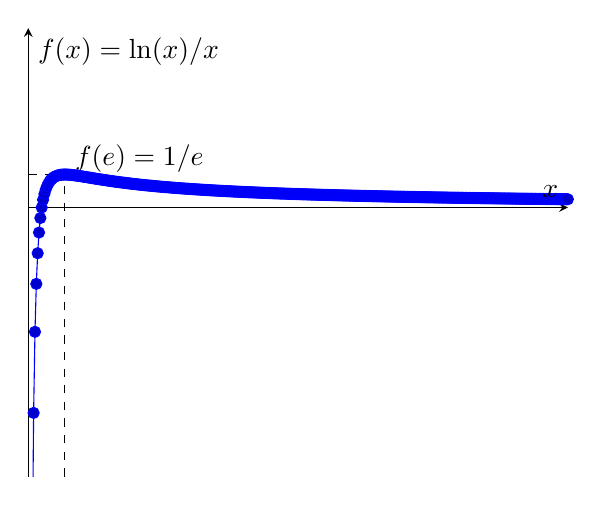
\begin{tikzpicture}[scale=1]
\begin{axis}[
  domain=0.1:100,
  samples=1000,
  axis lines=middle,
  xlabel={$x$}, ylabel={$f(x)=\ln(x)/x$},
  ymin=-3, ymax=2, xmin=0, xmax=40,
  ticks=none,
]
\addplot {ln(x)/x};
\addplot[dashed] coordinates {(2.71828,-3) (2.71828,0.367879)};

\addplot[dashed] coordinates {(0,0.367879) (6,0.367879)};
\node[anchor=west] at (axis cs:2.75,0.55) {$f(e)=1/e$};
\end{axis}
\end{tikzpicture}
\end{center}

\paragraph{Application à la comparaison de $\pi^{e}$ et $e^{\pi}$.}
Comparer $\pi^{e}$ et $e^{\pi}$ revient à comparer leurs logarithmes :
\[
\pi^{e} \;\underset{?}{\lessgtr}\; e^{\pi}
\quad\Longleftrightarrow\quad
e\ln(\pi) \;\underset{?}{\lessgtr}\; \pi \ln(e)
\quad\Longleftrightarrow\quad
\frac{\ln(\pi)}{\pi} \;\underset{?}{\lessgtr}\; \frac{ln(e)}{e}.
\]
Or $\pi>e$ et $f$ est \emph{décroissante} sur $(e,+\infty)$, donc
\[
f(\pi)=\frac{\ln\pi}{\pi} \;<\; f(e)=\frac{1}{e}.
\]
Par conséquent,
\[
\frac{\ln\pi}{\pi} < \frac{ln(e)}{e}
\;\Longleftrightarrow\;
e\ln\pi < \pi \ln(e)
\;\Longleftrightarrow\;
\boxed{\;\pi^{e} < e^{\pi}\; }.
\]

\subsection*{Méthode 2 :}


On utilise le développement de Taylor de $e^x$ :
\[
e^x \;=\; 1 + x + \frac{x^2}{2}\ +  \dots 
\]
Ainsi, pour tout $x\ne 0$,
\[
e^x \;>\; 1 + x.
\]
En particulier, avec 
\[
x \;=\; \frac{\pi}{e} - 1 \;>\; 0 \quad (\text{car } \pi>e),
\]
on obtient
\[
e^{\frac{\pi}{e}-1} \;>\; 1 + \left(\frac{\pi}{e}-1\right) \;=\; \frac{\pi}{e}.
\]
En multipliant par $e$ :
\[
e^{\frac{\pi}{e}} \;>\; \pi.
\]

Donc, 
\[
\boxed{\pi^{\,e} < e^{\,\pi}}.
\]

\section{Somme de taches divisible par $11$}

\begin{exerciseBox}[Somme de taches divisible par $11$]
On dispose de $101$ chiens dalmatiens (chiens blancs à taches noires).\\ 
Pour chaque chien $i$, on note $a_i \in \mathbb{N}$ le nombre de ses taches noires.
Montrer qu'il existe un \emph{sous-ensemble non vide} de ces chiens tel que la somme des taches noires soit divisible par $11$.
\end{exerciseBox}

\subsection*{Solution :}


On note
\[
C=\{A_1,\dots,A_{101}\},
\]
où $A_i$ est le $i$-ème chien dalmatien et $a_i\in\mathbb{N}$ le nombre de ses taches noires.

\medskip
\textbf{Cas 1.} Il existe $i$ tel que $a_i$ soit divisible par $11$. \\
Alors l’ensemble $\{A_i\}$ (un seul chien) convient : sa somme vaut $a_i\equiv 0 \pmod{11}$.

\medskip
\textbf{Cas 2.} Sinon, pour tout $j\in\{1,\dots,101\}$, $a_j$ n’est pas divisible par $11$. \\
Autrement dit, le reste de la division euclidienne de chaque $a_j$ par $11$ appartient à $\{1,\dots,10\}$.

\begin{rappelBox}[Principe des tiroirs (pigeonhole)]
Si l’on répartit $N$ objets dans $k$ boîtes, alors il existe au moins une boîte contenant au moins
\[
\left\lceil \frac{N}{k} \right\rceil
\]
objets.
\end{rappelBox}

Nous avons ici $N=101$ nombres et $k=10$ classes de congruence possibles (les restes $1,\dots,10$). Par le principe des tiroirs, il existe donc un reste $r\in\{1,\dots,10\}$ tel que \emph{au moins $11$} des $a_j$ vérifient $a_j\equiv r \pmod{11}$.

Considérons précisément $11$ de ces chiens, disons d’indices $j_1,\dots,j_{11}$, tous dans la même classe $r$ modulo $11$. Alors
\[
a_{j_1}+\cdots+a_{j_{11}} \equiv r+\cdots+r = 11\,r \equiv 0 \pmod{11}.
\]
Ainsi, la somme des $11$ nombres de cette sous-famille est un multiple de $11$, donc le sous-ensemble $\{A_{j_1},\dots,A_{j_{11}}\}$ convient.

\medskip
\textbf{Conclusion.} Dans tous les cas, il existe un sous-ensemble non vide de $C$ tel que la somme des nombres de taches noires des chiens qui le composent soit divisible par $11$.


